\documentclass[10pt]{article}
\usepackage{icmlko}

\icmlmeta{IP 파운데이션 월드모델}{136}{합친 순위는 집단 순서를 잰다}{표본을 늘리려 거름망을 풀었더니 $\rho$ 도 오르고 구간도 좁아졌다 --- 그리고 그 절반이 ``어느 무리인가''를 맞힌 것이었다}

\begin{document}

\twocolumn[
\icmlheader

\begin{abstract}
노트 135가 팝업 후행을 59에서 339로 늘려야 한다고 했다. \textbf{먼저 천장을
셌다} --- 지금 저장소는 모든 거름망을 풀어도 202건이 한계이고, 분할 시점
$T$를 옮겨도 75건이 최대다(그것도 학습을 잃는다). 남은 길은 거름망 완화
하나뿐이라 그 거래 조건을 쟀다. \textbf{그런데 거래가 아니었다.} 계수 방법
필터만 풀면 $n$이 59에서 116이 되면서 $\rho$가 $+$0.3688에서
$+$0.4562로 \emph{오르고} 반폭이 0.132에서 0.087로 \emph{좁아진다}. 양쪽이
다 좋아지는 순이득이다. \textbf{채택 직전에 갈랐다.} 116건을 계수 방법으로
가르면 검증 계수 59건이 $+$0.4495이고 주장 · 추정 57건이 $-$0.0756이다.
합친 값이 어떻게 둘 다보다 높은가 --- 두 무리의 \emph{수준}이 갈려 있기
때문이다. 주장 무리는 라벨 중앙이 3.073 대 2.661, 예측 중앙이 1.978 대
1.374로 체계적으로 높다($p\approx$2e$-$6). 집단 안 순위로 바꿔 집단 간
순서를 빼면 \textbf{$+$0.4562가 $+$0.2099로 무너진다.} 합친 $\rho$의 절반
이상이 ``이게 주장 라벨인가''를 맞힌 몫이었고, 그건 예측 과제가 아니다.
\textbf{같은 결함을 세 번째 만났다} --- 묶음(노트 127) · 폴드 평균(노트 131) ·
집단 수준(여기). 셋 다 ``부분집단이 갈려 있으면 합친 순위 상관이 집단 간
순서를 잰다''는 한 문장이다. 그래서 가드로 만들었다. 표지가 있으면 집단 안
순위로 다시 재고, 없으면 예측 중앙으로 가르되 \textbf{집단이 없을 때의 기대
감쇠를 모의로 빼고} 2 표준편차를 넘을 때만 적는다 --- 보정 없이 걸었더니
챔피언 설정을 잡았다.
\end{abstract}
]

\begin{figure*}[t]
\centering
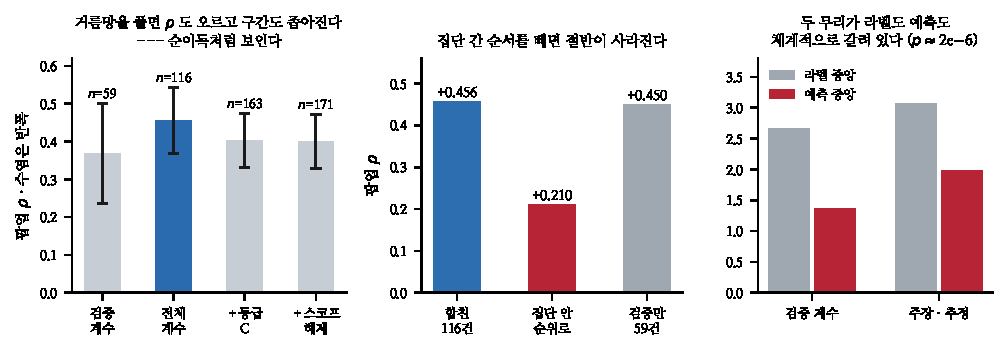
\includegraphics[width=\textwidth]{figs/group.pdf}
\caption{왼쪽 --- 거름망을 풀면 $\rho$도 오르고 구간도 좁아진다. 가운데 ---
집단 간 순서를 빼면 절반이 사라진다. 오른쪽 --- 두 무리의 수준차.}
\end{figure*}

\section{먼저 천장을 셌다}

노트 135가 $n\approx339$를 요구했다. 도달 가능한지부터 봤다.

\begin{table}[t]
\centering\tsize
\caption{거름망을 하나씩 풀 때 팝업 후행(2025$+$).}
\begin{tabular}{lr}
\toprule
현행 (A·B · 스코프 · 검증 계수) & 59 \\
계수 필터 풀기 & 116 \\
$+$ 등급 C까지 & 163 \\
$+$ 스코프 조건 풀기 & 171 \\
라벨만 있으면 & \textbf{202} \\
\bottomrule
\end{tabular}
\end{table}

\claimx{\textbf{339는 지금 저장소로 불가능하다.} 천장이 202다. 분할 시점
$T$를 앞으로 당기는 지렛대도 죽었다 --- 최대 75건이고(반폭 0.109) 팝업
학습이 0$\sim$1건으로 준다. 팝업 레코드가 2024$\sim$2026에 몰려 있어 옮길
앞쪽 질량이 없다.}{202건에서 예상 반폭이 0.065다 --- 지금의 절반이다.
도달할 수는 없어도 절반은 갈 수 있다는 뜻이라 거래 조건을 쟀다.}

\section{거래가 아니라 순이득처럼 보였다}

\begin{table}[t]
\centering\tsize
\caption{F9 짝 순위 · 기본 축. 반폭은 붓스트랩 800회.}
\begin{tabular}{lrrr}
\toprule
& $n$ & $\rho$ & 반폭 \\
\midrule
검증 계수 (현행) & 59 & $+$.3688 & .132 \\
\textbf{전체 계수} & 116 & \textbf{$+$.4562} & \textbf{.087} \\
$+$등급 C & 163 & $+$.4022 & .072 \\
$+$스코프 해제 & 171 & $+$.3995 & .071 \\
\bottomrule
\end{tabular}
\end{table}

둘째 줄이 현행보다 $\rho$도 높고 구간도 좁다. 라벨 품질을 표본과 맞바꾸는
거래일 줄 알았는데 양쪽이 다 좋아진다.

\section{채택 직전에 갈랐다}

노트 133이 주장 라벨을 ``예측 불가''라고 쟀던 것이 걸렸다. 그때는 검색 $+$
달력 축에서 $\rho$ 0.03이었다. 기본 축에서도 그런지 보고, 합친 값이 어떻게
나오는지 갈랐다.

\begin{table}[t]
\centering\tsize
\caption{116건을 계수 방법으로 가른 것. 같은 모형 · 같은 예측.}
\begin{tabular}{lrrr}
\toprule
& 합친 & 검증 (59) & 주장 (57) \\
\midrule
기본 축만 & $+$.4562 & $+$.4495 & \textbf{$-$.0756} \\
$+$검색$+$달력 & $+$.4053 & $+$.4300 & $+$.0297 \\
\bottomrule
\end{tabular}
\end{table}

합친 값이 두 부분 어느 쪽보다도 높다. 스피어만은 부분집합 값의 가중평균이
아니므로 산술적으로 불가능한 일은 아니다 --- 다만 그런 일이 생기려면
두 무리가 갈려 있어야 한다.

\claimx{\textbf{갈려 있다.} 주장 무리는 라벨 중앙이 3.073으로 검증 무리의
2.661보다 높고($p$=2.2e$-$6), 예측 중앙도 1.978 대 1.374로 높다
($p$=2.8e$-$7). 모형이 ``주장 라벨 건은 더 크다''를 맞히고 있고, 그것이
합친 순위에 들어간다.}{모형은 계수 방법을 안 본다 --- 축과 달력만 본다.
주장 라벨이 붙는 팝업이 실제로 더 큰 행사인 것으로 읽는다.}

\claimx{\textbf{집단 간 순서를 빼면 절반이 사라진다.} 각 무리 안에서 순위로
바꾼 뒤 다시 재면 $+$0.4562가 \textbf{$+$0.2099}가 된다. 검증만 쓴
$+$0.4495보다 훨씬 낮다. \textbf{116건 정의는 개선이 아니라 개악이다.}}{반폭이
좁아진 것도 같은 이유다 --- 집단 간 분리는 재표집에 안정적이라 구간을
좁힌다. \textbf{좁은 구간이 좋은 추정을 뜻하지 않는다.}}

\section{세 번째로 같은 결함이다}

\begin{table}[t]
\centering\tsize
\caption{모양이 같은 셋.}
\begin{tabular}{lll}
\toprule
& 갈린 것 & 증상 \\
\midrule
노트 127 & 축 없는 레코드 & 전부 같은 점수, $\rho$는 나옴 \\
노트 131 & 폴드 & 예측이 폴드 평균, 부호 뒤집힘 \\
노트 136 & 계수 방법 & 합친 $\rho$의 절반이 집단 순서 \\
\bottomrule
\end{tabular}
\end{table}

한 문장으로 줄면 이렇다. \textbf{부분집단이 갈려 있으면 합친 순위 상관은
집단 간 순서를 잰다.} 세 번 다 다른 자리에서 만났고 세 번 다 처음엔
좋은 소식으로 보였다.

\claimx{\textbf{가드로 만들었다(아홉째).} 집단 표지가 있으면 집단 안 순위로
다시 재고 차가 0.15를 넘으면 실패로 적는다. 표지가 없으면 예측 중앙으로
가르되, \textbf{집단이 없을 때의 기대 감쇠를 모의로 빼고} 2 표준편차를
넘을 때만 적는다.}{보정을 안 걸었더니 챔피언 설정을 잡았다 --- 예측
중앙에서 가르면 $X$ 분산이 반으로 줄어 집단이 없어도 상관이 준다. 참
$\rho$ 0.5 · $n$ 59에서 기대 차가 0.17이고 챔피언의 관측이 0.165였다.}

표지 없는 쪽은 검정력이 낮다. 이번 인공물도 중앙 분할로는 못 잡았다
--- 두 무리가 예측값에서 겹치기 때문이다. \textbf{표지가 있을 때만 제대로
잡힌다}는 것을 한계로 적어 둔다. 팝업은 계수 방법을 표지로 물려 놓았다.

\begin{table}[t]
\centering\tsize
\caption{새 가드를 지금 판에 걸어 본 것.}
\begin{tabular}{lrl}
\toprule
& 차 & \\
\midrule
현행 (검증 계수 59건) & $+$.033 & 통과 \\
확장 (전체 계수 116건) & $+$.211 & \textbf{실패} \\
\bottomrule
\end{tabular}
\end{table}

\section{남은 것}

\begin{table}[t]
\centering\tsize
\caption{다음.}
\begin{tabular}{ll}
\toprule
표본 & 202가 천장. 339는 새 레코드가 있어야 한다 \\
표지 & 다른 도메인에도 집단 표지를 찾아 물릴 것 \\
검정력 & 표지 없는 탐지는 못 잡는다 --- 개선 여지 \\
\bottomrule
\end{tabular}
\end{table}

첫 줄이 이 사이클의 결론이다. 노트 135가 요구한 339건은 지금 자료로 못
만들고, 만들 수 있는 202건은 방금 본 이유로 쓰면 안 된다. \textbf{팝업의
분해능은 새 레코드 없이는 안 올라간다.} 세 노트에 걸쳐 세 갈래(태깅 ·
계수 필터 · 분할 시점)를 다 재 봤고 셋 다 막혔다.

\end{document}
